
\section{Implementaci�n}
Con la fase de dise�o finalizada, se procede a realizar la fase de implementaci�n. Durante esta fase se genera el c�digo de la aplicaci�n y se genera el manual de usuario.

La aplicaci�n fue desarrollada en el lenguaje Java version 1.8. Con el fin de crear las interfaces de usuario se utilizo el Framework JavaFX.

En el cuadro~\ref{fig:actualizacion_implementacion} se presenta las tareas realizadas durante esta fase del desarrollo del software.

\begin{longtable}{||c| m{10cm}||}
  \caption{Actividades fase de implementaci�n}
  \label{fig:actualizacion_implementacion}
  \endfirsthead
  \hline
  N� Iteraci�n & Descripci�n\\ [0.5ex] 
  \hline\hline
  1 & Se codifican las clases para cargar la red \textit{Network}.\\
  \hline
  2 & Se codifican las clases del modulo metaheuristica. \newline Se implementa el Algoritmo Gen�tico.\newline Se implementa la codificaci�n del problema monoobjetivo \textit{Pipe Optimizing}. \newline Se implementan los operadores IntegerRandomMutation, SBXCrossover, IntegerPolinomialMutation, IntegerRangeRandomMutation y UniformSelection.\\
  \hline
  3 & Se implementan la interfaz de usuario principal. \newline Se implementa el componente para visualizar la red \newline Se implementa la interfaz de configuraci�n del problema. \newline Se implementa la interfaz de visualizaci�n de resultados de optimizaci�n. \newline Se implementa la interfaz que muestra el gr�fico con los resultados de la optimizacion. \newline Se implementa la funcionalidad para guardar las soluciones en TSV. \newline Se implementa funcionalidad para exportar la soluci�n escogida como un inp(Formato del archivo de configuraci�n de red). \\
  \hline
  4 & Se agrega el algoritmo NSGAII. \newline Se implementa la codificaci�n del problema multiobjetivo \textbf{Pumping Scheduling}.\\
  \hline
  5 & Se modifican las clases y archivos relacionados a la interfaces de usuario. \newline Se implementa la funcionalidad para realizar m�ltiples simulaciones independientes de un mismo algoritmo para los problemas multiobjetivos (Experimentos). \newline Se implementa la funcionalidad para realizar la simulaci�n usando los valores del archivo de red.\\
  \hline
  6 & Se modifica el componente de visualizaci�n de red para mostrar para cada tipo de elemento que conforma la red un s�mbolo distinto. \newline Se implementa funcionalidad para mostrar una leyenda de los s�mbolos. \newline Se implementa ventana de configuraci�n de la aplicaci�n. \newline Se implementa la funcionalidad para realizar m�ltiples simulaciones independientes para los problemas monoobjetivo (Se adapta para utilizar los Experimentos antes utilizados solo en problemas multiobjetivos).\newline Se permite agregar valores por defecto en la ventana de configuraci�n del problemas. \newline Se implementa la funcionalidad para exportar resultados a un Excel.\\
  \hline
\end{longtable}

A continuaci�n se presentara para cada una de las funcionalidades escogidas las interfaces implementadas.

\paragraph{Funcionalidad 1}: La Figura~\ref{fig:ventana_visualizacion} muestra la ventana de visualizaci�n de la red.

\begin{figure}[H]
  \centering
  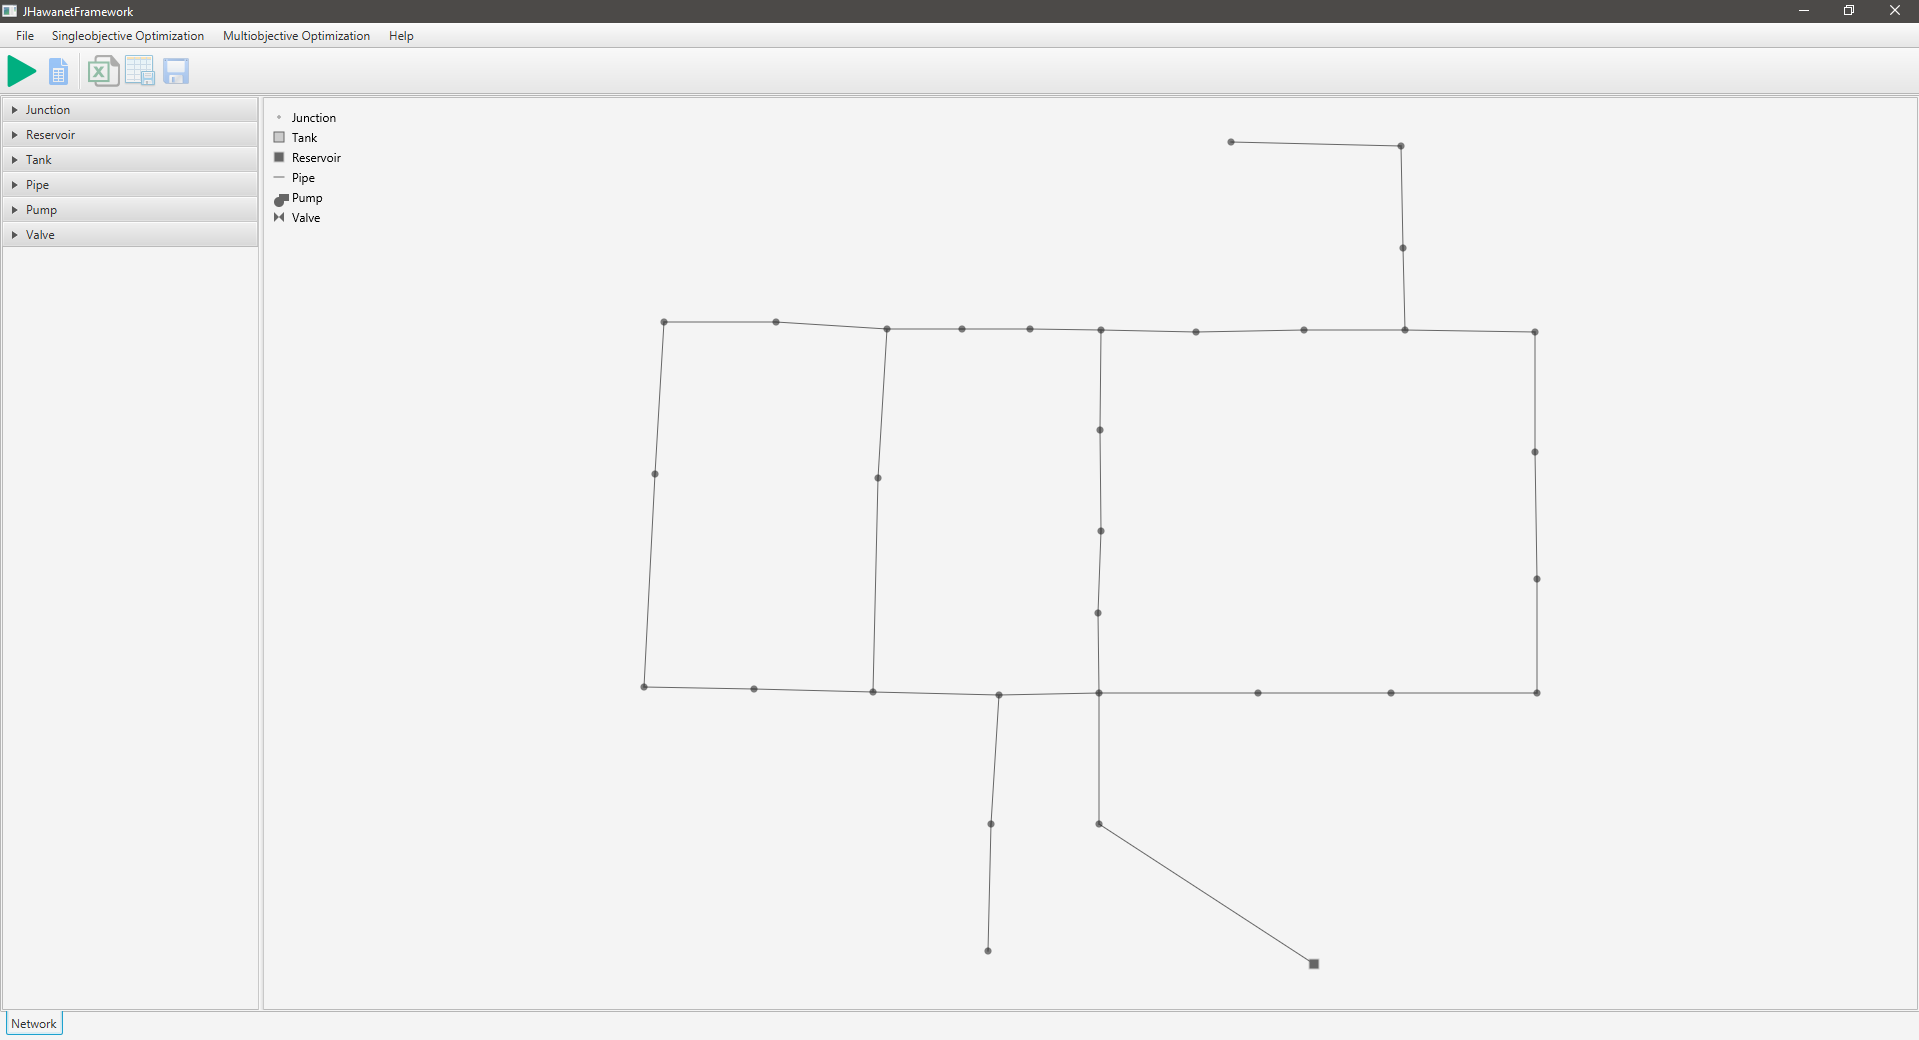
\includegraphics[width=\textwidth]{Capitulo4/assets/VisualizacionRed.png}
	\caption{Ventana principal de la aplicaci�n donde se visualiza la red}
	\label{fig:ventana_visualizacion}
\end{figure}

\paragraph{Funcionalidad 2}: Las Figuras~\ref{fig:ventana_descripcion},~\ref{fig:ventana_configuracion_problema},~\ref{fig:ventana_operador},~\ref{fig:ventana_retroalimentacion} y~\ref{fig:ventana_resultados_opt} muestran las ventana utilizadas durante el cumplimiento de esta funcionalidad.

\begin{figure}[H]
  \centering
  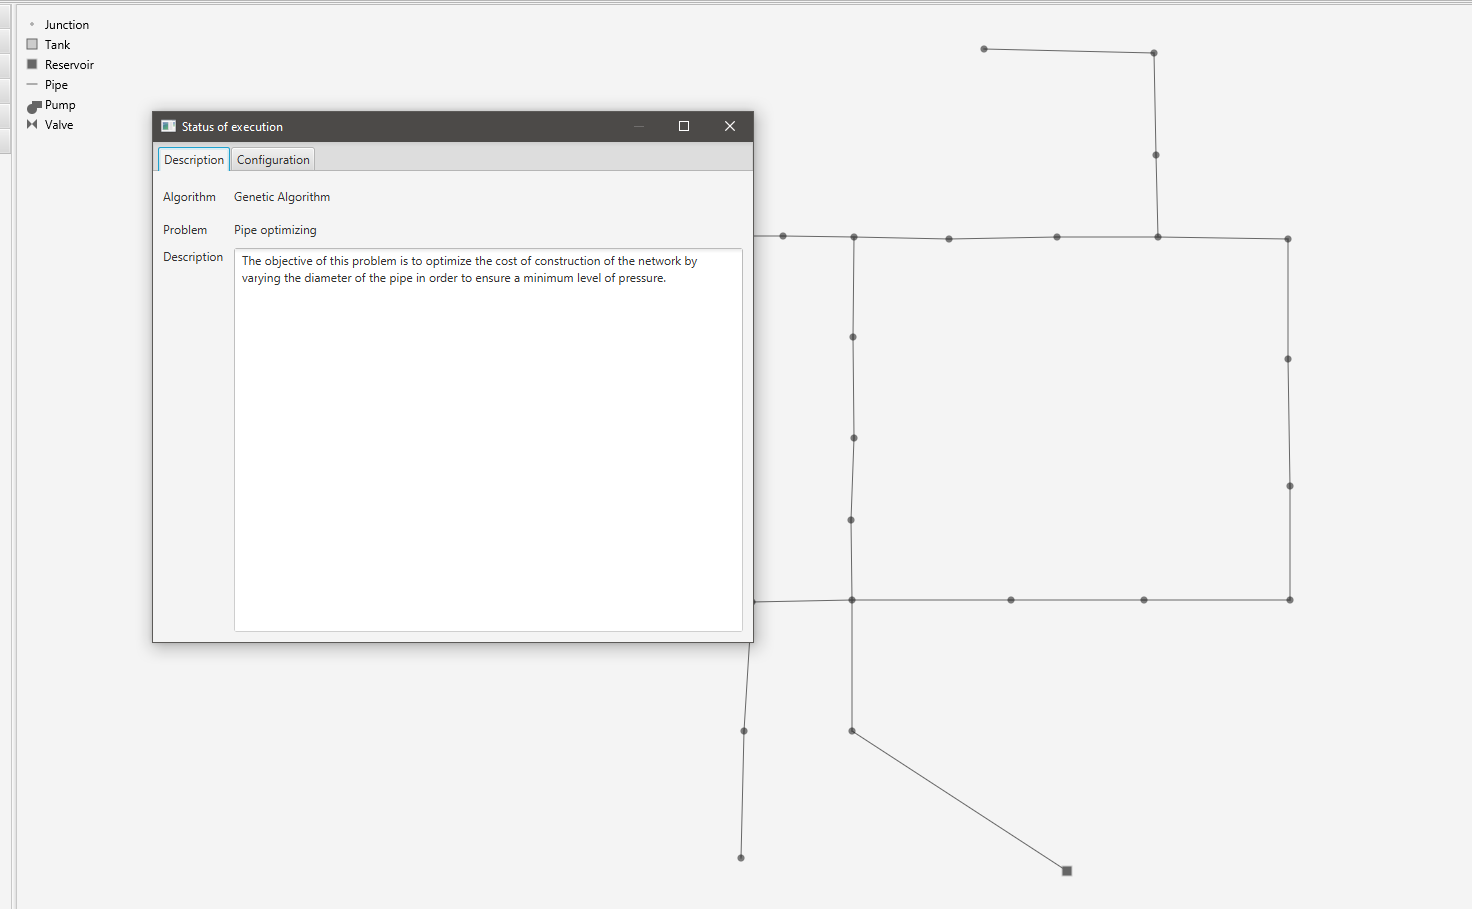
\includegraphics[width=\textwidth]{Capitulo4/assets/ConfiguracionProblema1.png}
	\caption{Ventana de descripci�n del problema.}
	\label{fig:ventana_descripcion}
\end{figure}

\begin{figure}[H]
  \centering
  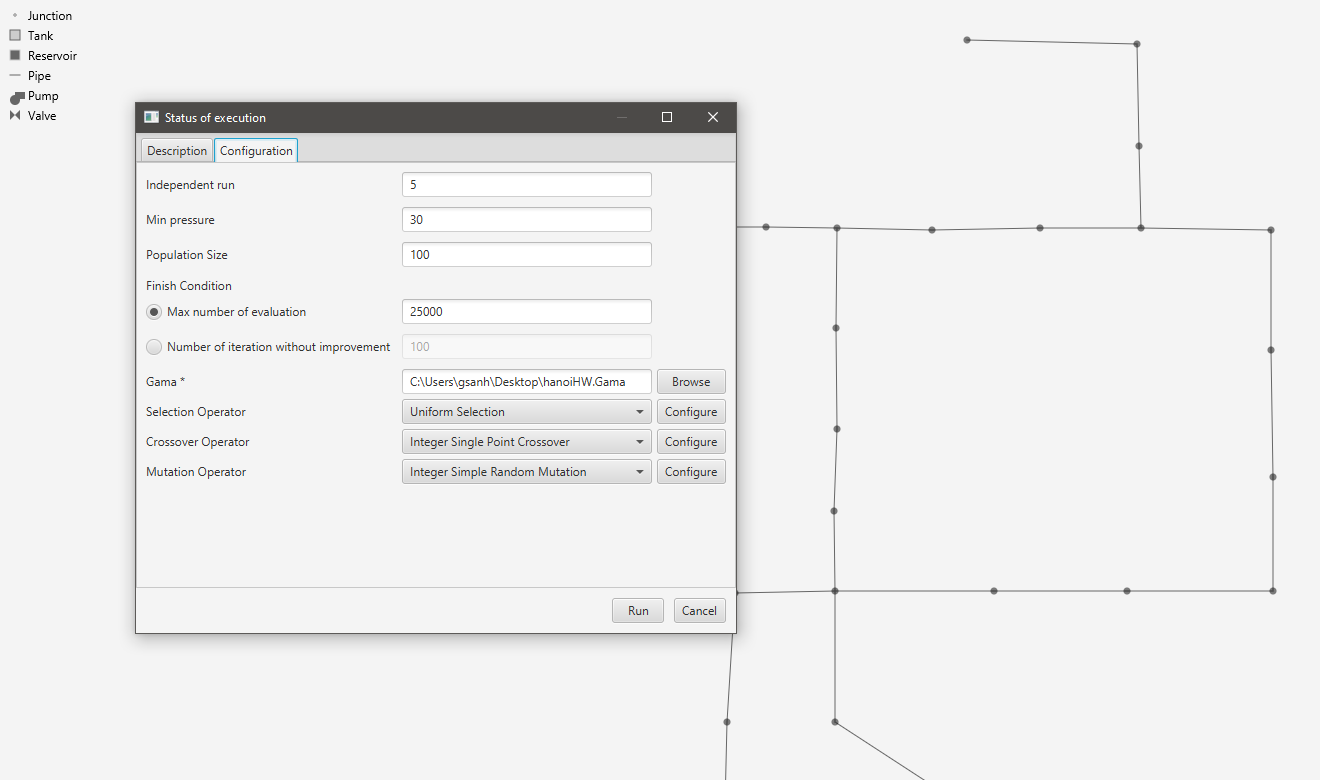
\includegraphics[width=\textwidth]{Capitulo4/assets/ConfiguracionProblema2.png}
	\caption{Ventana de configuraci�n del problema.}
	\label{fig:ventana_configuracion_problema}
\end{figure}

\begin{figure}[H]
  \centering
  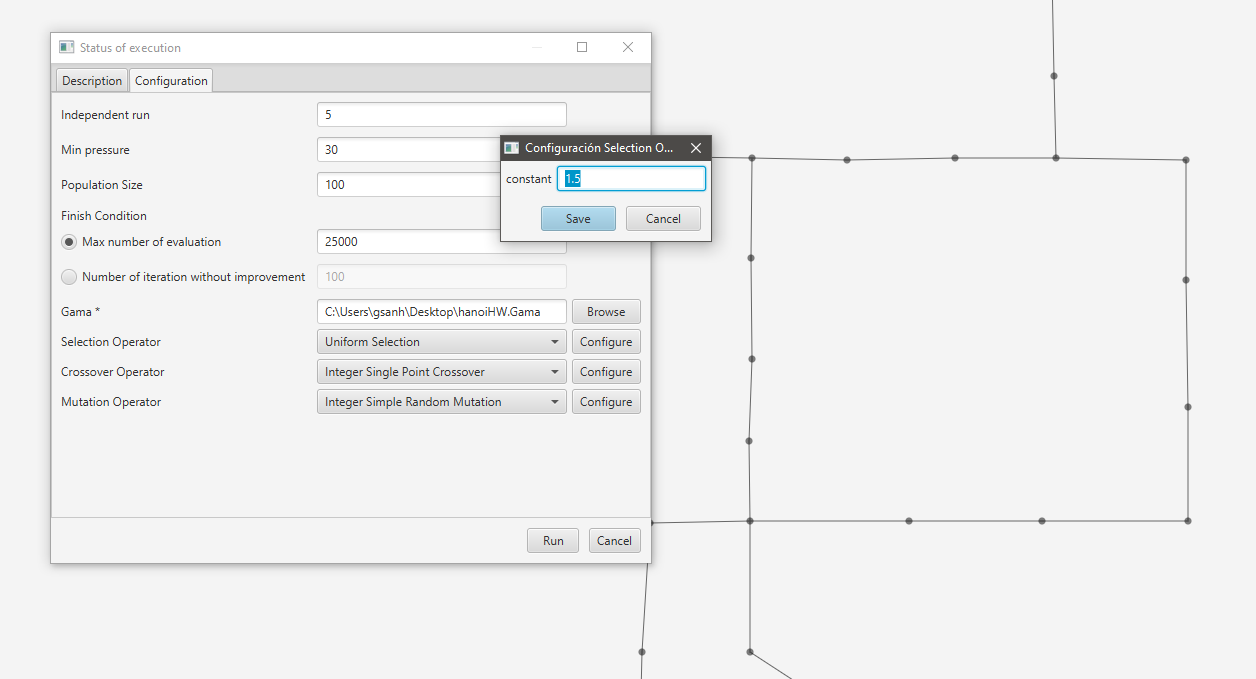
\includegraphics[width=\textwidth]{Capitulo4/assets/ConfiguracionProblema3.png}
	\caption{Ventana de configuraci�n de par�metros del operador \textit{UniformSelection}}
	\label{fig:ventana_operador}
\end{figure}

\begin{figure}[H]
  \centering
  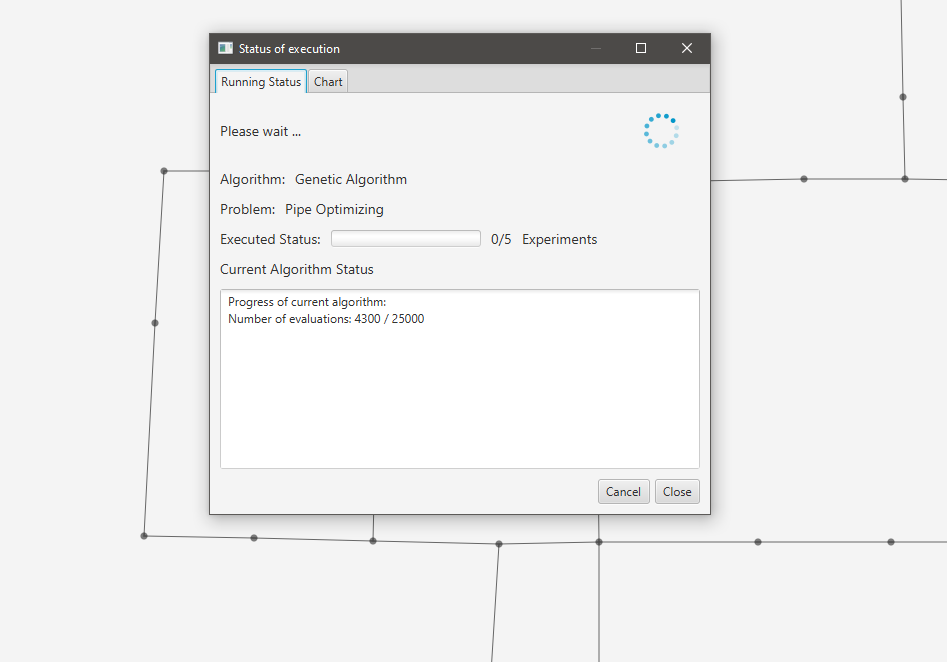
\includegraphics[width=\textwidth]{Capitulo4/assets/VentanaDeEjecucionMono.png}
	\caption{Ventana del retroalimentaci�n mostrada durante la ejecuci�n}
	\label{fig:ventana_retroalimentacion}
\end{figure}

\begin{figure}[H]
  \centering
  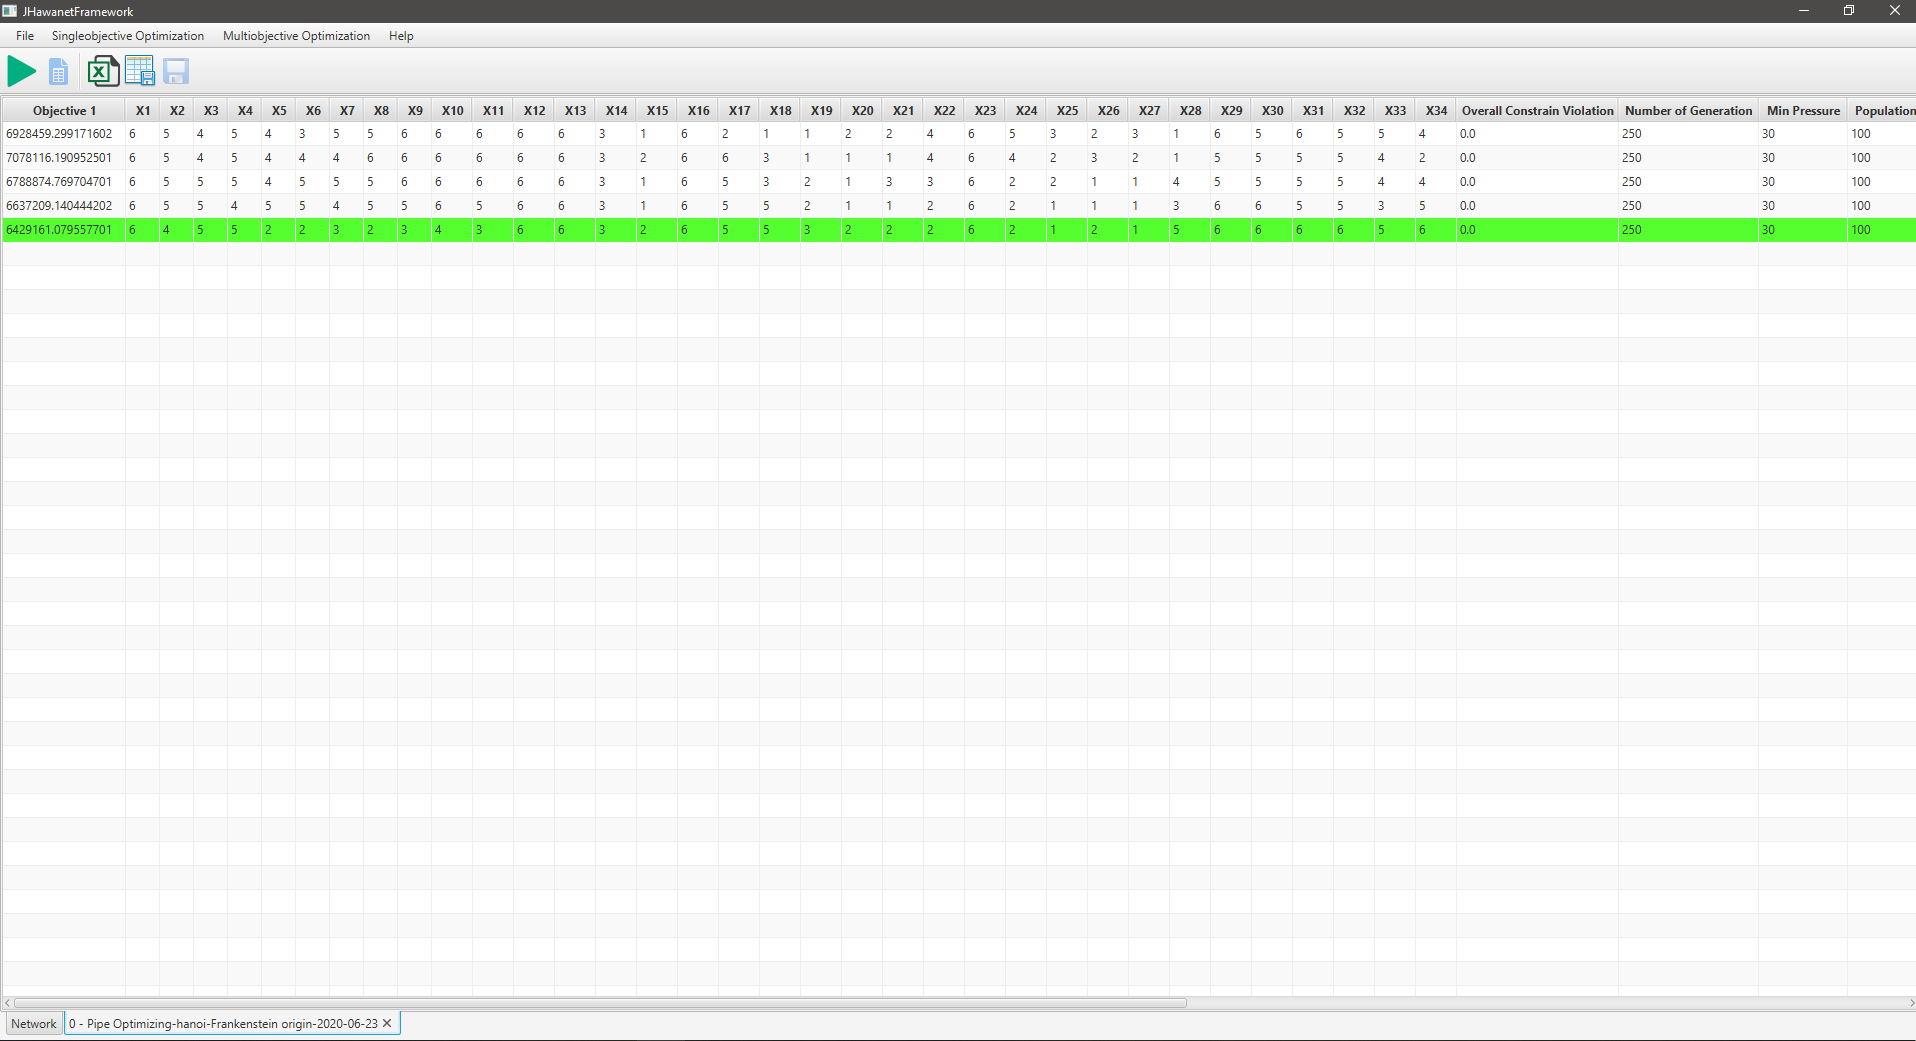
\includegraphics[width=\textwidth]{Capitulo4/assets/VentanaDeResultadosMono.png}
	\caption{Ventana de resultados generada cuando termina la ejecuci�n para el problema monoobjetivo Pipe Optimizing}
	\label{fig:ventana_resultados_opt}
\end{figure}

\paragraph{Funcionalidad 3}: La Figura~\ref{fig:ventana_simulacion_hyd} muestra la ventana con los resultados de una simulaci�n hidr�ulica para la red cargada.


\begin{figure}[H]
  \centering
  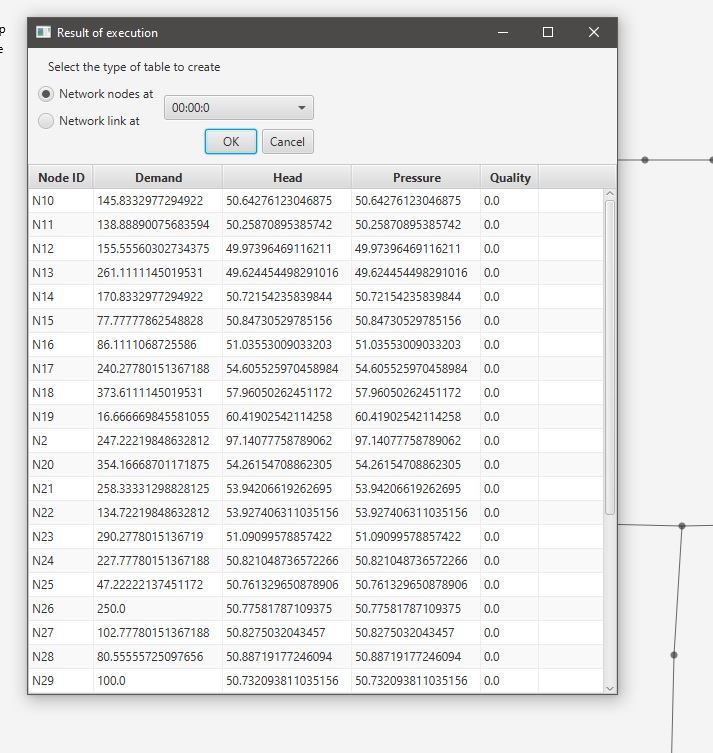
\includegraphics[width=\textwidth]{Capitulo4/assets/VentanaDeSimulacionHidraulica.png}
	\caption{Ventana de simulaci�n hidr�ulica utilizando los valores del archivo de red}
	\label{fig:ventana_simulacion_hyd}
\end{figure}